\chapter{Проектирование} \label{ch13}


\section{Анализ требований} \label{ch1:sec13}

Прежде чем приступить к написанию, необходимо определить, какой функционал требуется для реализации приложения. В своей основе программа работает с файловой системой и делает ее анализ. Управление приложением осуществляется пользователем через ввод определенных команд. Наиболее интересным является пункт, в котором требуется сделать сохранение истории запросов и результата поиска.

Продемонстрируем работу приложения при помощи диаграммы IDEF0 A-0 (рис 1.1).

\begin{figure}[ht] 
	\center
	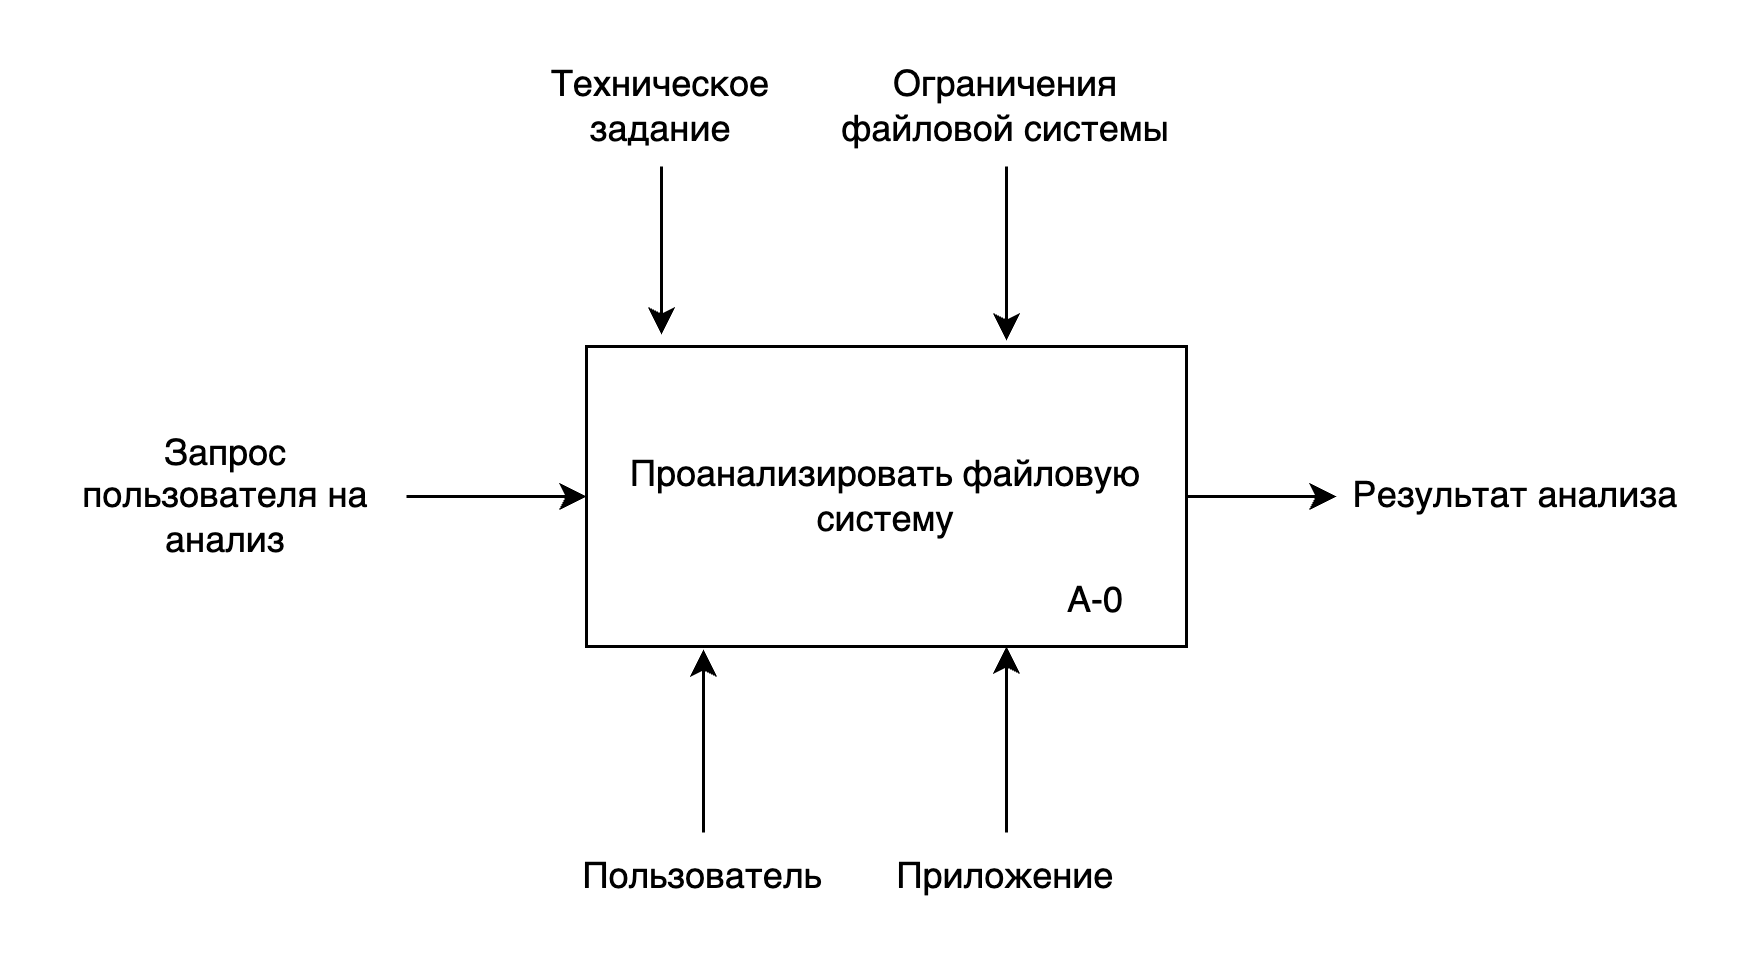
\includegraphics [scale=0.17] {my_folder/images/IDEF.png}
	\caption{диаграмма IDEF0 A-0} 
	\label{fig:idef0-A-0}  
\end{figure}

Конкретизируем блок «Проанализировать файловую систему». В сущности, эта задача представляет собой последовательность других задач:
\begin{enumerate}
	\item Проанализировать директорию. Пользователь выбирает конкретную директорию, вариант анализа и ожидает получить результат.
	\item Обработать ошибки. Работа с файловой системой связана с большим количеством возможных ошибок. Например, пользователь может указать неверный путь к директории, или у него может не быть прав, чтобы работать с тем или иным файлом.
	\item Сохранить историю в файл. Каждое действие в системе должно записываться в специальный файл. 
\end{enumerate}

\begin{figure}[ht] 
	\center
	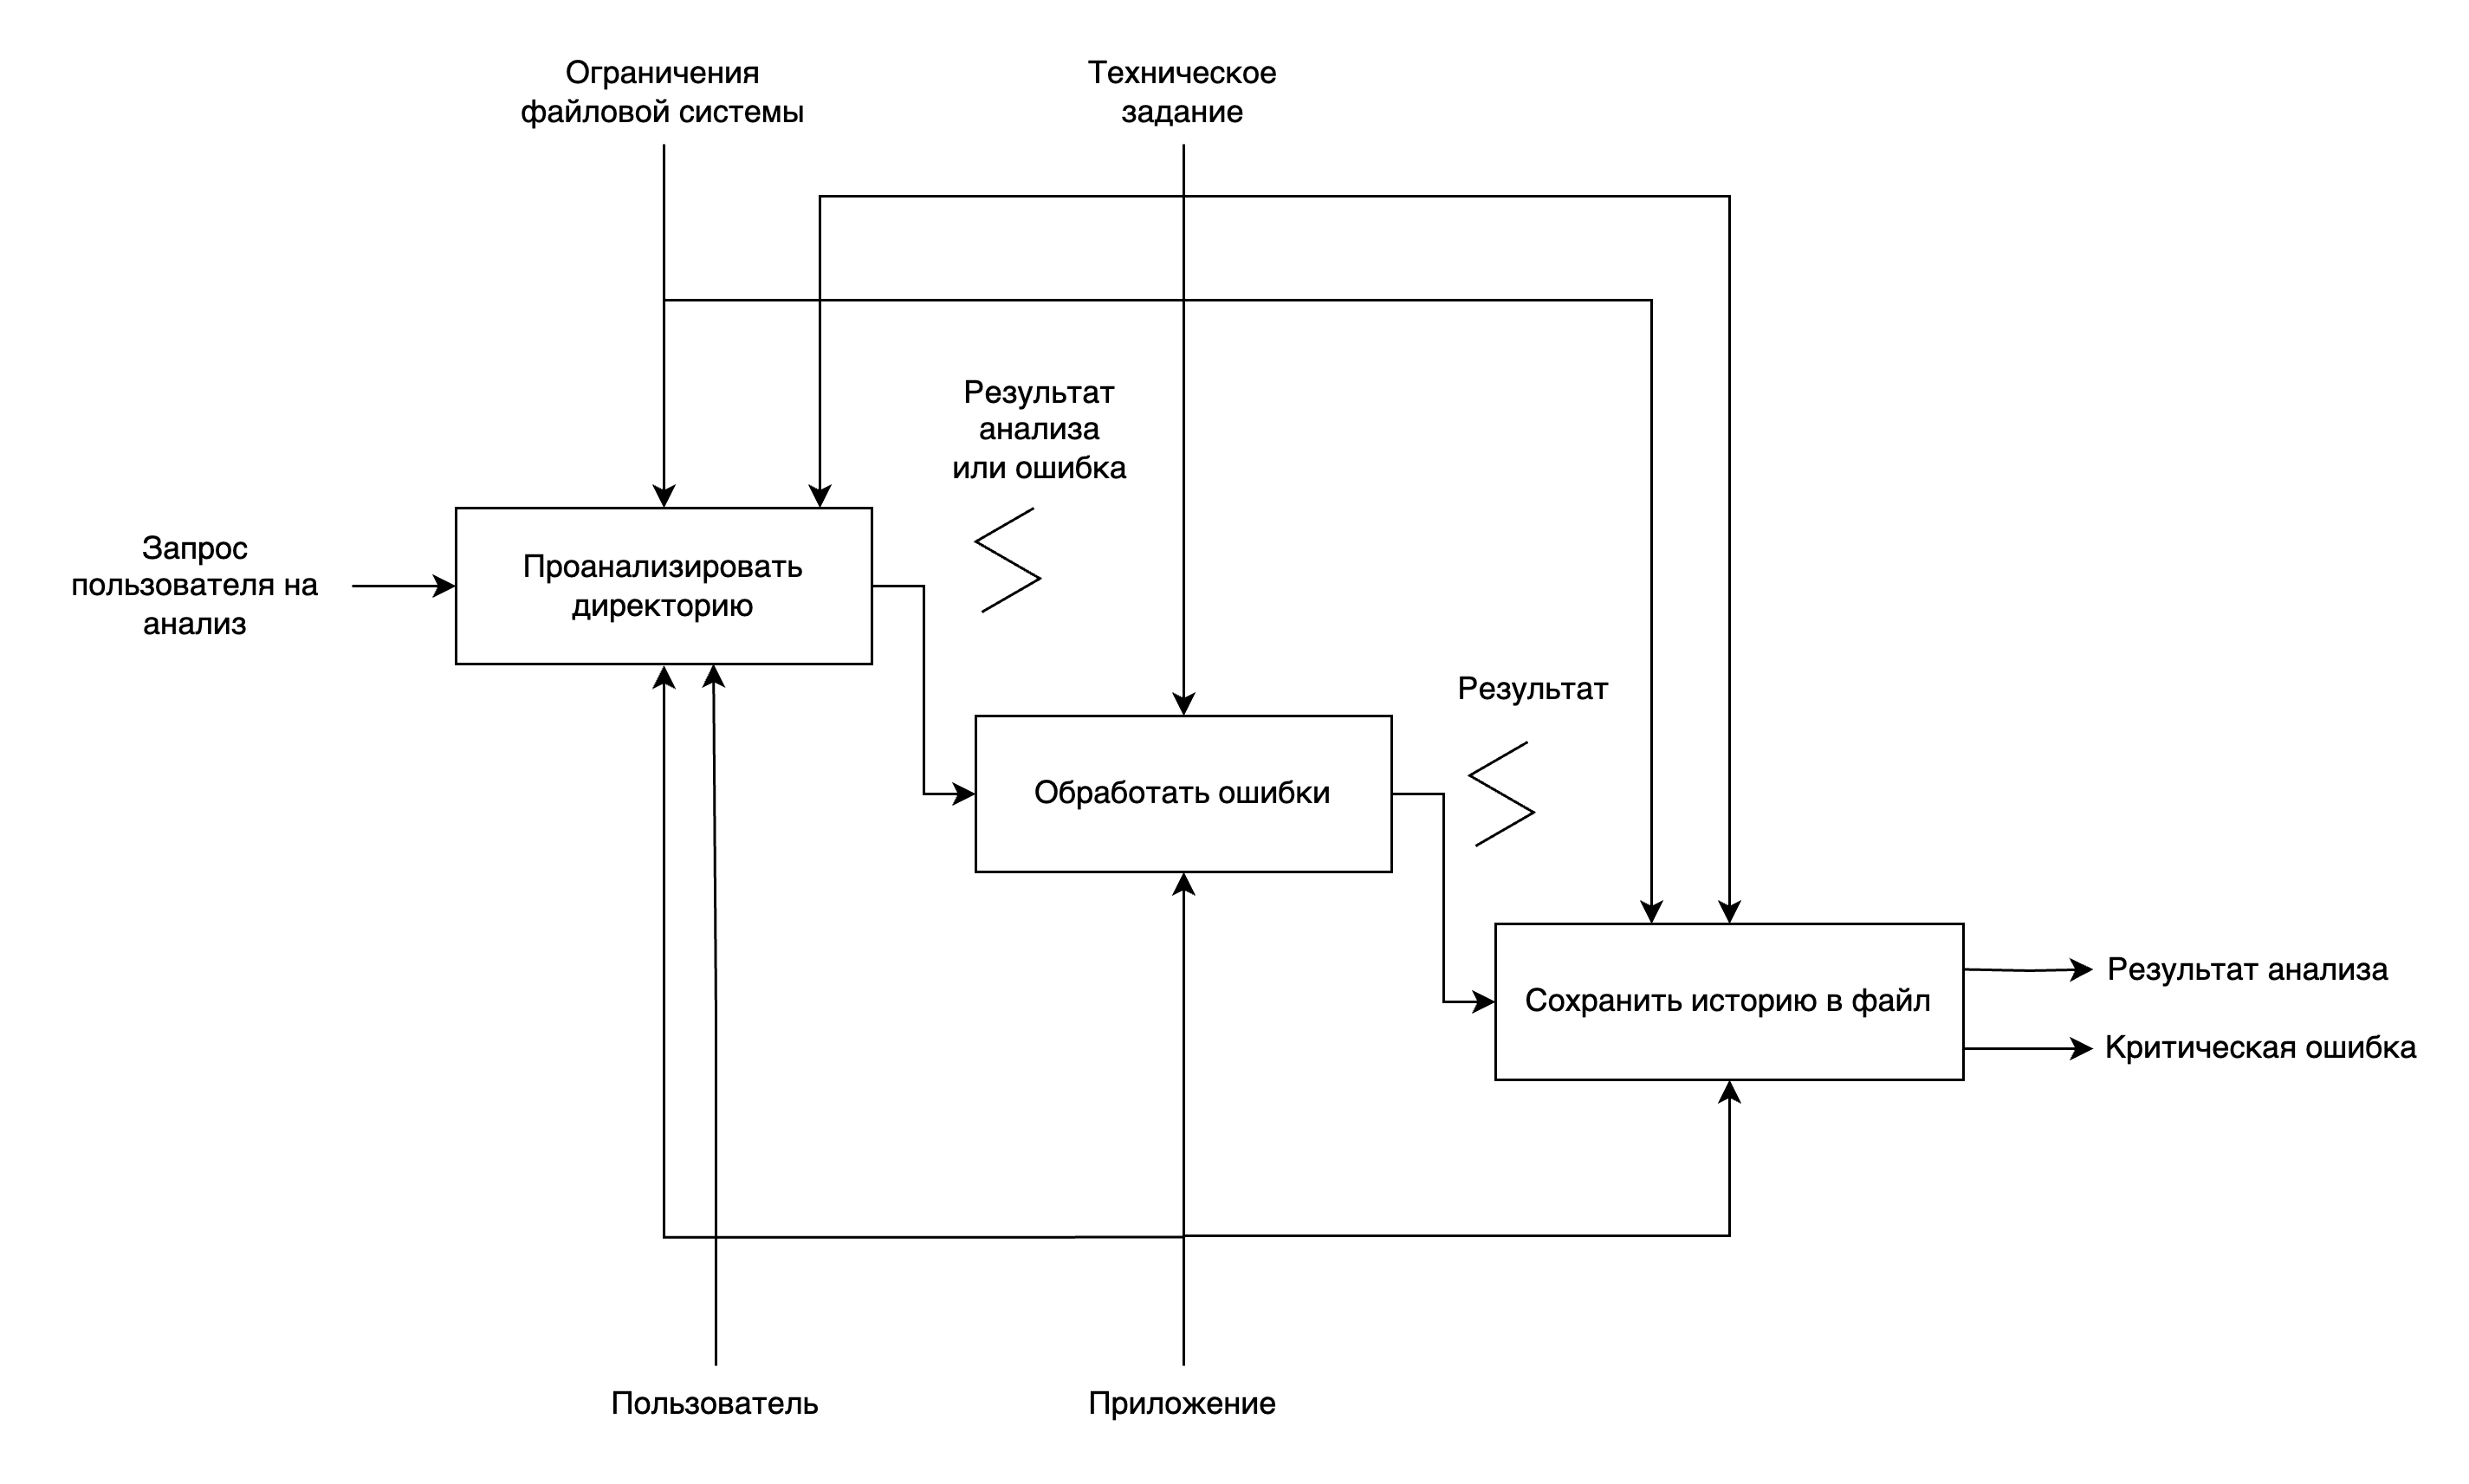
\includegraphics [scale=0.15] {my_folder/images/IDEF0_A0.png}
	\caption{диаграмма IDEF0 A0} 
	\label{fig:idef0-A0}  
\end{figure}


\newpage\section{Выбор архитектуры} \label{ch1:sec22}
%

Выбор архитектуры – очень важный этап. От него зависит, как пойдет дальнейшая разработка проекта. Хорошая архитектура позволяет очертить правильные границы приложения и облегчить процесс разработки.

Исходя из требований, для успешной реализации приложения нам стоит обратить внимание на событийно-ориентированную архитектуру. Кроме того, будет важно разделить приложение как на вертикальные, так и горизонтальные срезы.

Начнем проектировать приложение в следующем порядке:
\begin{enumerate}
	\item \textit{Доменная область} – работа с файловой системой. Этот компонент проекта является самым основным. К сожалению, язык C++ предоставляет хоть и гибкий, но не совсем удобный интерфейс для взаимодействия с файловой системой. Именно поэтому стоит разработать «обертку» над стандартным API языка для удобства взаимодействия.
	\item \textit{CQRS (Command and Query Responsibility Segregation)} – один из архитектурных паттернов, позволяющих разделить логику проекта на команды, запросы и ответы. Команды используются, когда приложение меняет свое состояние, запросы – для получения каких-то данных. Результаты всех этих операций приходят в ответах. В проекте мы реализуем упрощенную версию библиотеки. Кроме того, мы представим механизм конвейерной обработки запросов, который позволит работать с событиями, происходящими в системе. Такой подход не только позволит выполнить пункт с записью файл, но и даст дополнительные точки для расширения приложения, которые нам понадобятся.
	\item В \textit{инфраструктурных сервисах} будут находиться компоненты, работающие с вводом/выводом, а также абстракция приложения, декларирующая правила его работы, и компонент, отвечающий за ее удобное создание.
	\item \textit{Обработчики запросов} будут содержать логику для анализа файловой системы. Обобщая, все основные требования из технического задания будут находиться в этой части.
\end{enumerate}

\section{Проектирование интерфейса взаимодействия с файловой системой} \label{ch1:conclusion2}

Файловую систему будут представлять две модели – \textit{Директория} и \textit{Файл}. Для нашей задачи нам потребуется только информация о их названии, размере и последнем времени записи. Создадим следующие абстракции:

\begin{itemize}
	\item \verb|IFileSystemEntry| – интерфейс, содержащий методы \verb|name()|, \verb|size()|, \verb|updatedAt()| для получения информации о модели в файловой системе.
	\item \verb|DirectoryEntry| – директория. Класс, реализующий \verb|IFileSystemEntry| и содержащий методы \verb|subdirectories()| – поддиректории и \verb|files()| – файлы, находящиеся в этой директории.
	\item \verb|FileEntry| – файл. Класс, реализующий \verb|IFileSystemEntry|. Дополнительных методов и полей не содержит.
\end{itemize}

И \verb|DirectoryEntry|, и \verb|FileEntry| создаются при помощи конструктора, где указывается их полный путь. Однако он не всегда может быть указан верно, поэтому стоит предусмотреть механизм исключений в подобных ситуациях. Для этого создадим классы:

\begin{itemize}
	\item \verb|ApplicationException| – базовый класс для исключений в приложении. Содержит сообщение о возникновении ошибки.
	\item \verb|DirectoryNotFoundException| – наследник \verb|ApplicationException|. Сообщает о том, что директория не была найдена.
	\item \verb|FileNotFoundException| – наследник \verb|ApplicationException|. Сообщает о том, что файл не был найден.
\end{itemize}

\section{Проектирование CQRS библиотеки} \label{ch1:conclusion3}

CQRS библиотека необходима, чтобы разделить логику на запросы/ответы и их обработчиков. Также нам понадобится реализовать конвейер обработки запросов, в который можно будет встраивать свои компоненты, использующие и преобразующие запросы с ответами (например, запись о событиях в файл).

Стоит начать с интерфейсов:
\begin{itemize}
	\item \verb|IStringFormattable| – интерфейс, содержащий метод \verb|toString()|, который должен возвращать текстовое представление объекта.
	\item \verb|IRequest| – интерфейс-маркер запроса. Реализует \verb|IStringFormattable|.
	\item \verb|IResponse| – интерфейс-маркер ответа. Реализует \verb|IStringFormattable|.
	\item \verb|IRequestHandler| – интерфейс обработчика запроса. Содержит единственный метод \verb|IResponse* handle(IRequest& request)|, который выполняет обработку запроса, возвращая ответ.
	\item \verb|IGenericRequestHandler<TRequest, TReponse>| - шаблонный абстрактный класс обработчика запроса. Реализует \verb|IRequestHandler|. Содержит метод \verb|TResponse* handleRequest(TRequest& request)|, который также выполняет обработку запроса, но уже с более строгими моделями для запроса и ответа. Таким образом можно будет получать данные, содержащиеся в \verb|IRequest| сразу без преобразований типов. Переопределяет метод \verb|handle|, вызывая \verb|handleRequest| и передавая в него \verb|IRequest|, преобразованный к \verb|TRequest| через \verb|dynamic_cast|.
	\item \verb|IRequestSender| – интферфейс для отправки запросов. Содержит метод \verb|void send(IRequest& request)|.
	\item \verb|IRequestRouter| – роутер запросов, сопоставляющий тип запроса и его обработчик. Содержит метод \verb|getHandler(IRequest& request)|.
	\item \verb|IMiddleware| – элемент конвейера обработки. Содержит метод 
	\verb|IResponse* invoke(IRequest& request, RequestDelegate next)|. В нем можно считать запрос, переопределить ответ, вызывать следующий middleware через делегат next.
	\item \verb|RequestDelegate| – это алиас для \verb|std::function<IRespone(IRequest&)>|. Представляет собой вызов следующего Middleware в конвейере обработки.
\end{itemize}

\section{Проектирование инфраструктурных сервисов} \label{ch1:conclusion4}

Инфраструктурные сервисы позволят лаконично описать работу приложения, дополнительно обеспечив механизм инверсии зависимостей.
Начнем также с интерфейсов:
\begin{enumerate}
	\item \verb|ILogger| – абстракция, позволяющая записывать события. Содержит метод \verb|void log(std::string text)|.
	\item \verb|IUserInteractor| – интферфейс для взаимодействия с пользователем. Содержит метод \verb|bool shouldExit()|, сообщающий о том, что пользователь запросил выход из приложения. Самое главное – метод \verb|IRequest* readRequest()|. Благодаря CQRS библиотеки и полиморфизму подтипов мы можем считывать любые запросы пользователя вызовом всего лишь одного метода.
	\item \verb|Application| – абстракция приложения, описывающая, как оно будет работать. Содержит \verb|MiddlewarePipeline|, \verb|RequestHandler|, \verb|IUserInteractor| Позволяет расширять конвейер обработки при помощи метода \verb|void use(IMiddleware* middleware)|. Работа приложения запускается при помощи метода \verb|void run()|.
	\item \verb|ApplicationBuilder| – класс, позволяющий удобно создавать объект \verb|Application| через fluent интерфейс. Содержит методы на добавление \verb|IRequestRouter| и \verb|IUserInteractor|. По завершении настройки вызывается метод \verb|build()|, полностью инициализирующий объект Application.
\end{enumerate}

\newpage\section{Проектирование обработчиков запросов} \label{ch1:conclusion5}

Под конец, самая главная и сложная часть, где содержится основная логика из технического задания, становится самой легкой и шаблонизированной. Здесь мы используем подход featured-slice архитектуры, разделяя функциональность проекта на маленькие независимые детали. Это и есть те самые вертикальные срезы. Для каждой такой функциональности будет необходимо создать три класса – запрос, обработчик запроса, ответ. Так как все классы будут иметь одинаковую структуру, приведем только список возможностей, которые будут в проекте:

\begin{itemize}
	\item \verb|CountDirectories| - подсчет директорий в директории
	\item \verb|CountFiles| - подсчет файлов в директории
	\item \verb|CountTotalSize| - подсчет суммарного размера файлов в директоии
	\item \verb|FindDuplicates| - поиск файлов-дубликатов
	\item \verb|LargestFiles| - поиск самых больших файлов
	\item \verb|NewestFiles| - поиск самых новых файлов
\end{itemize}








